\subsection{Unknown-Onset Continuous Evidence: Scope and Failure Modes}
\label{sec:continuous-evidence}

The continuous component is evaluated separately from the prospective batch bank. Two completed development campaigns, H03 and H04, each contain three 80-s event parents with six successive load/line interventions and one normal parent. The same schedules are paired across nominal, in-bank R/X, and out-of-bank mixed R/X conditions. Thus each campaign contains 18 unique interventions and 54 paired event realizations. All use F01 operation, one instrumental-noise level, eight fixed PMUs, and the known nine-load/nine-line catalog. Neither campaign demonstrates unseen-source generalization. They are now development evidence and cannot be reused as a new blind confirmation.

In H03, R11 obtains \ContPriorTimely{}/54 correct family/source decisions before physical restoration, with \ContPriorExtras{} unmatched alarms. Table~\ref{tab:continuous-h04} reports the subsequent H04 outcomes. R11 retains \ContMixTimely{}/\ContMixTotal{} timely decisions, whereas its nominal ablation retains \ContNomTimely{}/\ContNomTotal{}. The mixture has fewer extras (\ContMixExtras{} versus \ContNomExtras{}), but loses one timely attribution. Parameter uncertainty therefore yields a trade-off, not uniform dominance. Under out-of-bank R/X, timely BUS31 attribution is \ContMixBusTimely{}/3 for the mixture and \ContNomBusTimely{}/3 for the nominal ablation. Eventual correct attribution would conceal that delay.

\begin{table}[t]
\centering\small
\caption{Executed continuous-stream development evidence (H04). Timely means correct family/source emitted before physical restoration; extras are unmatched alarms. OUT denotes out-of-bank R/X; F1 is report-level detection F1. These are paired realizations of 18 events from three event parents, not 54 independent events.}
\label{tab:continuous-h04}
\resizebox{\columnwidth}{!}{%
\begin{tabular}{lrrrr}
\toprule
Method & Timely & Extras & OUT timely & OUT F1\\
\midrule
R11 mixture & 53/54 & 4 & 17/18 & 0.818\\
R11 nominal & 54/54 & 7 & 18/18 & 0.828\\
Admission ablation & 52/54 & 0 & 16/18 & 0.854\\
ExtraTrees reference & 27/54 & 3 & 9/18 & 0.619\\
ExtraTrees short & 27/54 & 3 & 9/18 & 0.626\\
\bottomrule
\end{tabular}}
\end{table}


\begin{figure*}[t]
\centering
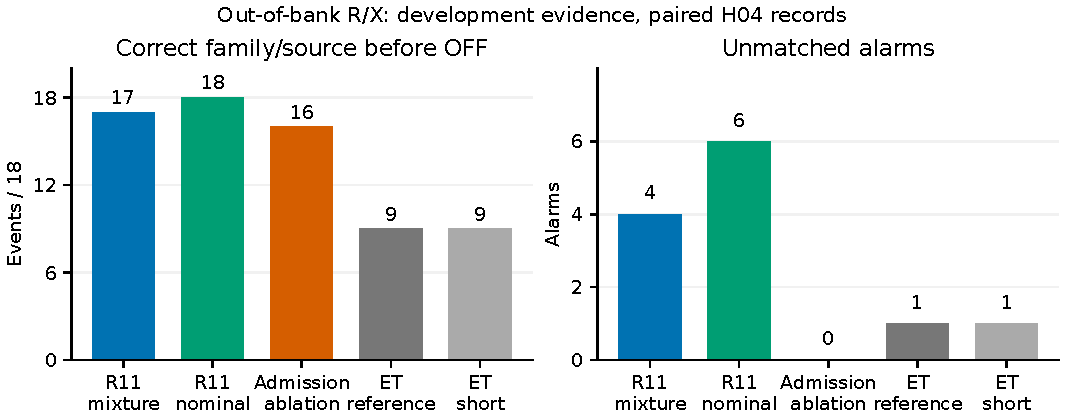
\includegraphics[width=0.92\textwidth]{figures/generated/continuous_tradeoff.pdf}
\caption{Failure trade-off under out-of-bank network error in H04. An additional causal-admission ablation eliminates unmatched alarms but rejects a real BUS16 intervention; the nominal R11 retains every timely event but has more extra alarms. These paired development results do not establish a universally superior variant.}
\label{fig:continuous-tradeoff}
\end{figure*}

An additional admission ablation retains \ContAdmissionTimely{}/\ContAdmissionTotal{} timely decisions with \ContAdmissionExtras{} extras. Its zero-extra result is insufficient for promotion: it rejects a true BUS16 load intervention whose retrospective onset lacks the required early witness. The change reduces public alarms while leaving the inherited physical states and hypothesis masses unchanged. We retain it as negative evidence rather than silently replacing R11. Both R11 references are now frozen; no bus-specific correction follows these observations.

The two frozen ExtraTrees adaptations obtain \ContETTimely{}/\ContMixTotal{} timely decisions here. This is an identical-stream causal comparison under the restricted load/line contract, not a recomputation of the hackathon leaderboard or an assertion about all event classes. Report-level F1 and event-level timely attribution measure different targets and are shown separately. The short normal exposure and three event parents cannot support a precise operational false-alarm rate or generalization confidence interval.

The published physical comparator passes equation-level tests for the reduced network, partial-observation marginalization, Gaussian log-likelihood, suffix-max recursion, angle wrapping, and stopping localization. On independently generated three-bus sequences under its own Gaussian law, \ChenMatchedCorrect{}/\ChenMatchedTotal{} post-change trials stop after onset at the correct line; \ChenMatchedEarly{} trial stops before the change. No alarm occurs over \ChenNormalExposure{} normal increments, with every normal sequence right-censored at its observation horizon. This checks an implementation under matched assumptions, not the numerical results of the original article. On three previously opened F01 normal records, the adapter alarms in all three; colored noise and frame dynamics violate its assumed law. We preserve that mismatch result and make no general superiority claim from it.

The confirmatory C01 configuration is sealed before its new draw. It specifies independent physical parents, longer normal records, paired R/X conditions, two instrumental-noise scales, persistent-line eligibility for the published comparator, and paired parent-cluster intervals. Both R11 references and both ExtraTrees artifacts remain fixed. Solver rejects, inference failures, late decisions, and right-censoring remain in the ledger. C01 has not been executed; it contributes no performance number to this manuscript. Source-disjoint inference, changing PMUs, faults, generation interventions, and the complete joint estimator remain outside this confirmatory contract.
